\subsection{球极投影}

考察点 \(e_{n}=(0,\ldots,0,1)\) （\(S_{n-1}\) 的），以及方程为 \(x_{n}=0\) 的、与向量 \(e_{n}\) 垂直的超平面 H。对每个点 \(x=(x_{i})\) （\(S_{n-1}\) 的，异于 \(e_{n}\) 的），使它对应于点 y，这里 y 是过 \(e_{n}\) 与 x 的直线和超平面 H 的交点（图 3）。容易验证，我们有

\[
\mathbf {y} = \frac {1}{1 - x _ {n}} (\mathbf {x} - x _ {n} \mathbf {e} _ {n})
\]

以及

\[
\boldsymbol {x} = \frac {\left| \left| \boldsymbol {y} \right| \right| ^ {2} - 1}{\left| \left| \boldsymbol {y} \right| \right| ^ {2} + 1} \boldsymbol {e} _ {n} + \frac {2}{\left| \left| \boldsymbol {y} \right| \right| ^ {2} + 1} \boldsymbol {y}.
\]

\pandocbounded{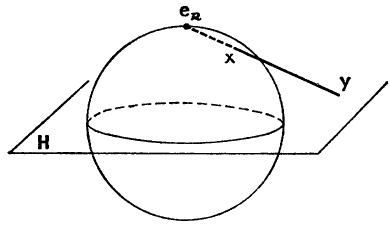
\includegraphics[keepaspectratio]{images/part001_990d2877.jpg}}\\
图 3.

若用 A 表示 \(\{e_{n}\}\) 在 \(S_{n-1}\) 中的补集，这些公式表明我们就这样定义了 A 到超平面 H 上的一个同胚。这个同胚称为 A 到 H 上的球极投影，或（滥用地说）\(S_{n-1}\) 到 H 上的球极投影；\(e_{n}\) 是投影的顶点，H 是投影超平面。更一般地，若 \(H'\) 是过 o 的任一超平面（\(B_{n}\) 的一个直径超平面），且 a 是 \(S_{n-1}\) 与过 o 而垂直于 \(H'\) 的直线的交点之一，我们就可以同样地定义以 a 为顶点、以 \(H'\) 为投影超平面的球极投影；在任何情形下，这个投影都可以通过一个把 \(H'\) 变成 H、把 a 变成 \(e_{n}\) 的正交变换化归为前一个投影。

命题 4. 若 \(n > 1\) ，欧氏球面 \(S_{n-1}\) 同胚于添加一个“无穷远点”而紧化的空间 \(\mathbf{R}^{n-1}\)（第 I 章，§ 9，第 8 小节，定理 4）。

因为球极投影定义了 \(S_{n-1}\) 中一点的补集到 \(R^{n}\) 的一个超平面上的同胚，而这个超平面同胚于 \(R^{n-1}\)。

推论 1. 球面 \(S_{n}\) 同胚于把球 \(B_{n}\) 中球面 \(S_{n-1}\) 的所有点等同起来所得到的商空间。

球 \(B_{n}\) 是正则空间（第 I 章，§ 8，第 4 小节）；因此 \(B_{n}\) 的商空间 F——把 \(S_{n-1}\) 的所有点等同起来而得到的——是豪斯多夫的（第 I 章，§ 8，第 6 小节，命题 15）。由于 \(B_{n}\) 是紧的，F 也是紧的，从而由亚历山德罗夫定理（第 I 章，§ 9，第 8 小节，定理 4），F 同胚于添加一个无穷远点而紧化的 n 维开球。因此结论由命题 2 与命题 4 得出。

推论 2. 圆周 \(\mathbf{S}_1\) 同胚于环面 \(\mathbf{T}\)。

在第 VIII 章，§ 2，第 1 小节中，我们将作为一个更精确的定理的推论重新得到这个结果。

命题 5. 若 \(n > 1\) ，欧氏球面 \(\mathbf{S}_{n-1}\) 是连通的且局部连通的，并且它的每个点都有一个同胚于 \(\mathbf{R}^{n-1}\) 的开邻域。

\(S_{n-1}\) 中一点的补集是连通的稠密集，因此（第 I 章，§ 11，第 1 小节，命题 1）\(S_{n-1}\) 是连通的。要看出每个点都有一个同胚于 \(R^{n-1}\) 的邻域，只需从一个异于该给定点的顶点作球极投影即可。

由这个命题以及第 3 小节的命题 3 推出，\(\mathbf{R}_n^*\) 作为两个连通空间的乘积是连通的（第 I 章，§ 11，第 4 小节，命题 8；参见 § 1，习题 10）。

\(S_{n-1}\) 与 \(B_{n}\) 的一个直径超平面所决定的闭（相应地，开）半空间的交，称为 \(S_{n-1}\) 的闭（相应地，开）半球面。通过到该直径超平面上的球极投影，不含投影顶点的闭（相应地，开）半球面被映成一个 n - 1 维的闭（相应地，开）球，从而同胚于它。

当 n = 2 时，我们说“半圆周”而不说“半球面”。

